\documentclass{scrreprt}

\usepackage{aligned-overset}
\usepackage{amsmath}
\usepackage{amsthm}
\usepackage{amssymb}
\usepackage{bm}
\usepackage[shortlabels]{enumitem}
\usepackage{hyperref}
\usepackage[utf8]{inputenc}
\usepackage{multicol}
\usepackage{mathtools}
\usepackage{pdflscape}
\usepackage{physics}
\usepackage{polynom}
\usepackage{tabularx}
\usepackage[table]{xcolor}
\usepackage{titling}
\usepackage{fancyhdr}
\usepackage{xfrac}
\usepackage{pgfplots}

\pgfplotsset{compat = newest}
\usetikzlibrary{arrows, arrows.meta}
\usetikzlibrary{calc}

\author{Karsten Lehmann \\ 4935758}
\date{WiSe 2024/25}
\title{Nachbereitungsaufgaben 10\\INF-B-110, Diskrete Strukturen}

\setlength{\headheight}{26pt}
\pagestyle{fancy}
\fancyhf{}
\lhead{\thetitle}
\rhead{\theauthor}
\lfoot{\thedate}
\rfoot{Seite \thepage}

\newcommand{\ggT}[0]{\text{ggT}}
\DeclarePairedDelimiter{\floor}{\lfloor}{\rfloor}

\begin{document}
\paragraph{N10} Gegeben sind die Graphen $G_1$ und $G_2$ durch je ein Diagramm:

\begin{minipage}{.45\textwidth}
  \begin{tikzpicture}
    \node[circle, draw, inner sep=0pt, minimum size=1mm,label=below:{1}] (1) at (0,0) {};
    \node[circle, draw, inner sep=0pt, minimum size=1mm,label=below:{2}] (2) at (1,0) {};
    \node[circle, draw, inner sep=0pt, minimum size=1mm,label=above:{3}] (3) at (1,1.5) {};
    \node[circle, draw, inner sep=0pt, minimum size=1mm,label=above:{4}] (4) at (0,1.5) {};
    \node[circle, draw, inner sep=0pt, minimum size=1mm,label=above:{5}] (5) at (2,0.75) {};
    \node[circle, draw, inner sep=0pt, minimum size=1mm,label=above:{6}] (6) at (3,0.75) {};
    \node[circle, draw, inner sep=0pt, minimum size=1mm,label=below:{7}] (7) at (3.5,0) {};
    \node[circle, draw, inner sep=0pt, minimum size=1mm,label=right:{8}] (8) at (4,0.75) {};
    \node[circle, draw, inner sep=0pt, minimum size=1mm,label=above:{9}] (9) at (3.5,1.5) {};

    \draw (1) -- (2) -- (3) -- (4);
    \draw (3) -- (5) -- (2);
    \draw (5) -- (6) -- (8) -- (7) -- (6) -- (9) -- (8);

    \node at (1, -1) {Graph $G_1$};
  \end{tikzpicture}
\end{minipage}
\begin{minipage}{.45\textwidth}
  \begin{tikzpicture}
    \node[circle, draw, inner sep=0pt, minimum size=1mm,label=below:{1}] (1) at (0, 0) {};
    \node[circle, draw, inner sep=0pt, minimum size=1mm,label=below:{2}] (2) at (1, 0) {};
    \node[circle, draw, inner sep=0pt, minimum size=1mm,label=below:{3}] (3) at (2, 0) {};
    \node[circle, draw, inner sep=0pt, minimum size=1mm,label=below:{4}] (4) at (3, 0) {};
    \node[circle, draw, inner sep=0pt, minimum size=1mm,label=left:{5}] (5) at (1, 1) {};
    \node[circle, draw, inner sep=0pt, minimum size=1mm,label=right:{6}] (6) at (2, 1) {};
    \node[circle, draw, inner sep=0pt, minimum size=1mm,label=above:{7}] (7) at (0, 2) {};
    \node[circle, draw, inner sep=0pt, minimum size=1mm,label=above:{8}] (8) at (1.5, 2) {};
    \node[circle, draw, inner sep=0pt, minimum size=1mm,label=above:{9}] (9) at (3, 2) {};

    \draw (1) -- (2) -- (5) -- (6) -- (8) -- (5);
    \draw (2) -- (3) -- (6);
    \draw (3) -- (4) -- (9) -- (8) -- (7) -- (1);

    \node at (1, -1) {Graph $G_2$};
  \end{tikzpicture}
\end{minipage}

\begin{enumerate}[(a)]
\item Sind diese Graphen zweifach zusammenhängend?
  Begründen Sie Ihre Antwort!
  Geben Sie im Falle, dass der Graph zweifach zusammenhängend ist,
  eine Ohrendekomposition an.
  (Zeigen Sie jeden Schritt durch Angabe eines Diagramms)

  \subparagraph{Lsg.} Der Graph $G_1$ ist nicht zweifach zusammenhängend, da er
  die Gelenkpunkte $2$, $3$, $5$ und $6$ enthält.
  Hingegen enthält der Graph $G_2$ keine Gelenkpunkte und ist somit zweifach
  zusammenhängend.

  Zur Ohrenzerlegung von $G_2$:
  \begin{enumerate}[1)]
  \item Starte mit einem Kreis:

    \begin{tikzpicture}
      \node[circle, draw, inner sep=0pt, minimum size=1mm,label=below:{1}] (1) at (0, 0) {};
      \node[circle, draw, inner sep=0pt, minimum size=1mm,label=below:{2}] (2) at (1, 0) {};
      \node[circle, draw, inner sep=0pt, minimum size=1mm,label=below:{3}] (3) at (2, 0) {};
      \node[circle, draw, inner sep=0pt, minimum size=1mm,label=below:{4}] (4) at (3, 0) {};
      \node[circle, draw, inner sep=0pt, minimum size=1mm,label=left:{5}] (5) at (1, 1) {};
      \node[circle, draw, inner sep=0pt, minimum size=1mm,label=right:{6}] (6) at (2, 1) {};
      \node[circle, draw, inner sep=0pt, minimum size=1mm,label=above:{7}] (7) at (0, 2) {};
      \node[circle, draw, inner sep=0pt, minimum size=1mm,label=above:{8}] (8) at (1.5, 2) {};
      \node[circle, draw, inner sep=0pt, minimum size=1mm,label=above:{9}] (9) at (3, 2) {};

      \draw (1) -- (2) -- (5) -- (6) -- (3) -- (4) -- (9) -- (8) -- (7) -- (1);
    \end{tikzpicture}

  \item Füge das \colorbox{green!20}{erste Ohr} hinzu

    \begin{tikzpicture}
      \node[circle, draw, inner sep=0pt, minimum size=1mm,label=below:{1}] (1) at (0, 0) {};
      \node[circle, draw, inner sep=0pt, minimum size=1mm,label=below:{2}] (2) at (1, 0) {};
      \node[circle, draw, inner sep=0pt, minimum size=1mm,label=below:{3}] (3) at (2, 0) {};
      \node[circle, draw, inner sep=0pt, minimum size=1mm,label=below:{4}] (4) at (3, 0) {};
      \node[circle, draw, inner sep=0pt, minimum size=1mm,label=left:{5}] (5) at (1, 1) {};
      \node[circle, draw, inner sep=0pt, minimum size=1mm,label=right:{6}] (6) at (2, 1) {};
      \node[circle, draw, inner sep=0pt, minimum size=1mm,label=above:{7}] (7) at (0, 2) {};
      \node[circle, draw, inner sep=0pt, minimum size=1mm,label=above:{8}] (8) at (1.5, 2) {};
      \node[circle, draw, inner sep=0pt, minimum size=1mm,label=above:{9}] (9) at (3, 2) {};

      \draw (1) -- (2) -- (5) -- (6) -- (3) -- (4) -- (9) -- (8) -- (7) -- (1);
      \draw[black!10!green, line width = 1mm] (2) -- (3);
    \end{tikzpicture}

  \item Füge das \colorbox{blue!20}{zweite Ohr} hinzu

    \begin{tikzpicture}
      \node[circle, draw, inner sep=0pt, minimum size=1mm,label=below:{1}] (1) at (0, 0) {};
      \node[circle, draw, inner sep=0pt, minimum size=1mm,label=below:{2}] (2) at (1, 0) {};
      \node[circle, draw, inner sep=0pt, minimum size=1mm,label=below:{3}] (3) at (2, 0) {};
      \node[circle, draw, inner sep=0pt, minimum size=1mm,label=below:{4}] (4) at (3, 0) {};
      \node[circle, draw, inner sep=0pt, minimum size=1mm,label=left:{5}] (5) at (1, 1) {};
      \node[circle, draw, inner sep=0pt, minimum size=1mm,label=right:{6}] (6) at (2, 1) {};
      \node[circle, draw, inner sep=0pt, minimum size=1mm,label=above:{7}] (7) at (0, 2) {};
      \node[circle, draw, inner sep=0pt, minimum size=1mm,label=above:{8}] (8) at (1.5, 2) {};
      \node[circle, draw, inner sep=0pt, minimum size=1mm,label=above:{9}] (9) at (3, 2) {};

      \draw (1) -- (2) -- (5) -- (6) -- (3) -- (4) -- (9) -- (8) -- (7) -- (1);
      \draw[black!10!green, line width = 1mm] (2) -- (3);
      \draw[black!10!blue, line width = 1mm] (5) -- (8);
    \end{tikzpicture}

  \item Füge das \colorbox{red!20}{dritte Ohr} hinzu

    \begin{tikzpicture}
      \node[circle, draw, inner sep=0pt, minimum size=1mm,label=below:{1}] (1) at (0, 0) {};
      \node[circle, draw, inner sep=0pt, minimum size=1mm,label=below:{2}] (2) at (1, 0) {};
      \node[circle, draw, inner sep=0pt, minimum size=1mm,label=below:{3}] (3) at (2, 0) {};
      \node[circle, draw, inner sep=0pt, minimum size=1mm,label=below:{4}] (4) at (3, 0) {};
      \node[circle, draw, inner sep=0pt, minimum size=1mm,label=left:{5}] (5) at (1, 1) {};
      \node[circle, draw, inner sep=0pt, minimum size=1mm,label=right:{6}] (6) at (2, 1) {};
      \node[circle, draw, inner sep=0pt, minimum size=1mm,label=above:{7}] (7) at (0, 2) {};
      \node[circle, draw, inner sep=0pt, minimum size=1mm,label=above:{8}] (8) at (1.5, 2) {};
      \node[circle, draw, inner sep=0pt, minimum size=1mm,label=above:{9}] (9) at (3, 2) {};

      \draw (1) -- (2) -- (5) -- (6) -- (3) -- (4) -- (9) -- (8) -- (7) -- (1);
      \draw[black!10!green, line width = 1mm] (2) -- (3);
      \draw[black!10!blue, line width = 1mm] (5) -- (8);
      \draw[black!10!red, line width = 1mm] (6) -- (8);
    \end{tikzpicture}
  \end{enumerate}
\item Geben Sie die Blockdekomposition dieser Graphen an, indem Sie jeweils
  \begin{itemize}
  \item alle Blöcke des Graphen durch je ein Diagramm zeichnen,
  \item die Knotenmenge, die Kantenmenge und ein Diagramm des Blockgraphen angeben.
  \end{itemize}

  \subparagraph{Lsg.}
  \begin{itemize}
  \item[Für $G_1$:] Der Graph besitzt die Blöcke
    \begin{enumerate}[$b_1$]
    \begin{minipage}{0.45\textwidth}
      \item \phantom{\null}

        \begin{tikzpicture}
          \node[circle, draw, inner sep=0pt, minimum size=1mm,label=below:{1}] (1) at (0,0) {};
          \node[circle, draw, inner sep=0pt, minimum size=1mm,label=below:{2}] (2) at (1,0) {};

          \draw (1) -- (2);
        \end{tikzpicture}

      \item \phantom{\null}

        \begin{tikzpicture}
          \node[circle, draw, inner sep=0pt, minimum size=1mm,label=above:{3}] (3) at (1,1.5) {};
          \node[circle, draw, inner sep=0pt, minimum size=1mm,label=above:{4}] (4) at (0,1.5) {};

          \draw (3) -- (4);
        \end{tikzpicture}

      \item \phantom{\null}

        \begin{tikzpicture}
          \node[circle, draw, inner sep=0pt, minimum size=1mm,label=below:{2}] (2) at (1,0) {};
          \node[circle, draw, inner sep=0pt, minimum size=1mm,label=above:{3}] (3) at (1,1.5) {};
          \node[circle, draw, inner sep=0pt, minimum size=1mm,label=above:{5}] (5) at (2,0.75) {};

          \draw (2) -- (3) -- (5) -- (2);
        \end{tikzpicture}
    \end{minipage}
    \begin{minipage}{0.45\textwidth}
      \item \phantom{\null}

        \begin{tikzpicture}
          \node[circle, draw, inner sep=0pt, minimum size=1mm,label=above:{5}] (5) at (2,0.75) {};
          \node[circle, draw, inner sep=0pt, minimum size=1mm,label=above:{6}] (6) at (3,0.75) {};

          \draw (5) -- (6);
        \end{tikzpicture}

      \item \phantom{\null}

        \begin{tikzpicture}
          \node[circle, draw, inner sep=0pt, minimum size=1mm,label=above:{6}] (6) at (3,0.75) {};
          \node[circle, draw, inner sep=0pt, minimum size=1mm,label=below:{7}] (7) at (3.5,0) {};
          \node[circle, draw, inner sep=0pt, minimum size=1mm,label=right:{8}] (8) at (4,0.75) {};
          \node[circle, draw, inner sep=0pt, minimum size=1mm,label=above:{9}] (9) at (3.5,1.5) {};

          \draw (6) -- (8) -- (7) -- (6) -- (9) -- (8);
        \end{tikzpicture}
    \end{minipage}
    \end{enumerate}

    Weiter besitzt $G_1$ die Gelenkpunkte $2$, $3$, $5$ und $6$.
    Somit hat der Blockgraph von $G_1$ die Knotenmenge
    \[
      V = \qty\big{b_1, b_2, b_3, b_4, b_5, 2, 3, 5, 6}
    \]
    und die Kantenmenge
    \[
      E = \qty{
        \qty\big{b_1, 2},
        \qty\big{b_2, 3},
        \qty\big{b_3, 2},
        \qty\big{b_3, 3},
        \qty\big{b_3, 5},
        \qty\big{b_4, 5},
        \qty\big{b_4, 6},
        \qty\big{b_5, 6}
      }
    \]
    Schließlich ist das Diagramm des Blockgraphen von $G_1$:

    \begin{tikzpicture}
      \node[circle, draw, inner sep=0pt, minimum size=1mm,label=below:{$b_1$}] (b1) at (0,0) {};
      \node[circle, draw, inner sep=0pt, minimum size=1mm,label=below:{2}] (2) at (1,0) {};
      \node[circle, draw, inner sep=0pt, minimum size=1mm,label=above:{$b_2$}] (b2) at (0,1) {};
      \node[circle, draw, inner sep=0pt, minimum size=1mm,label=above:{3}] (3) at (1,1) {};
      \node[circle, draw, inner sep=0pt, minimum size=1mm,label=above:{$b_3$}] (b3) at (1.5,0.5) {};
      \node[circle, draw, inner sep=0pt, minimum size=1mm,label=above:{5}] (5) at (2.5,0.5) {};
      \node[circle, draw, inner sep=0pt, minimum size=1mm,label=above:{$b_4$}] (b4) at (3.5,0.5) {};
      \node[circle, draw, inner sep=0pt, minimum size=1mm,label=above:{6}] (6) at (4.5,0.5) {};
      \node[circle, draw, inner sep=0pt, minimum size=1mm,label=above:{$b_5$}] (b5) at (5.5,0.5) {};

      \draw (b1) -- (2) -- (b3);
      \draw (b2) -- (3) -- (b3) -- (5) -- (b4) -- (6) -- (b5);
    \end{tikzpicture}

  \item[Für $G_2$:] Wie in Teilaufgabe (a) bestimmt, ist der Graph bereits
    zweifach zusammenhängend und somit ein Block.
    Nennen wir diesen Block im Folgenden $b_1$:

    \begin{tikzpicture}
      \node[circle, draw, inner sep=0pt, minimum size=1mm,label=below:{1}] (1) at (0, 0) {};
      \node[circle, draw, inner sep=0pt, minimum size=1mm,label=below:{2}] (2) at (1, 0) {};
      \node[circle, draw, inner sep=0pt, minimum size=1mm,label=below:{3}] (3) at (2, 0) {};
      \node[circle, draw, inner sep=0pt, minimum size=1mm,label=below:{4}] (4) at (3, 0) {};
      \node[circle, draw, inner sep=0pt, minimum size=1mm,label=left:{5}] (5) at (1, 1) {};
      \node[circle, draw, inner sep=0pt, minimum size=1mm,label=right:{6}] (6) at (2, 1) {};
      \node[circle, draw, inner sep=0pt, minimum size=1mm,label=above:{7}] (7) at (0, 2) {};
      \node[circle, draw, inner sep=0pt, minimum size=1mm,label=above:{8}] (8) at (1.5, 2) {};
      \node[circle, draw, inner sep=0pt, minimum size=1mm,label=above:{9}] (9) at (3, 2) {};

      \draw (1) -- (2) -- (5) -- (6) -- (8) -- (5);
      \draw (2) -- (3) -- (6);
      \draw (3) -- (4) -- (9) -- (8) -- (7) -- (1);
    \end{tikzpicture}

    Somit hat der Blockgraph von $G_2$ die Knotenmenge $V = \qty\big{b_1}$ und
    die Kantenmenge $E = \emptyset$.
    Das Diagramm des Blockgraphen ist schließlich \\

    \begin{tikzpicture}
      \node[circle, draw, inner sep=0pt, minimum size=1mm,label=below:{$b_1$}] (1) at (0, 0) {};
    \end{tikzpicture}
  \end{itemize}
\end{enumerate}
\end{document}
